\section{FMM3d Class Reference}
\label{classFMM3d}\index{FMM3d@{FMM3d}}
{\tt \#include $<$fmm3d.hpp$>$}

Inheritance diagram for FMM3d::\begin{figure}[H]
\begin{center}
\leavevmode
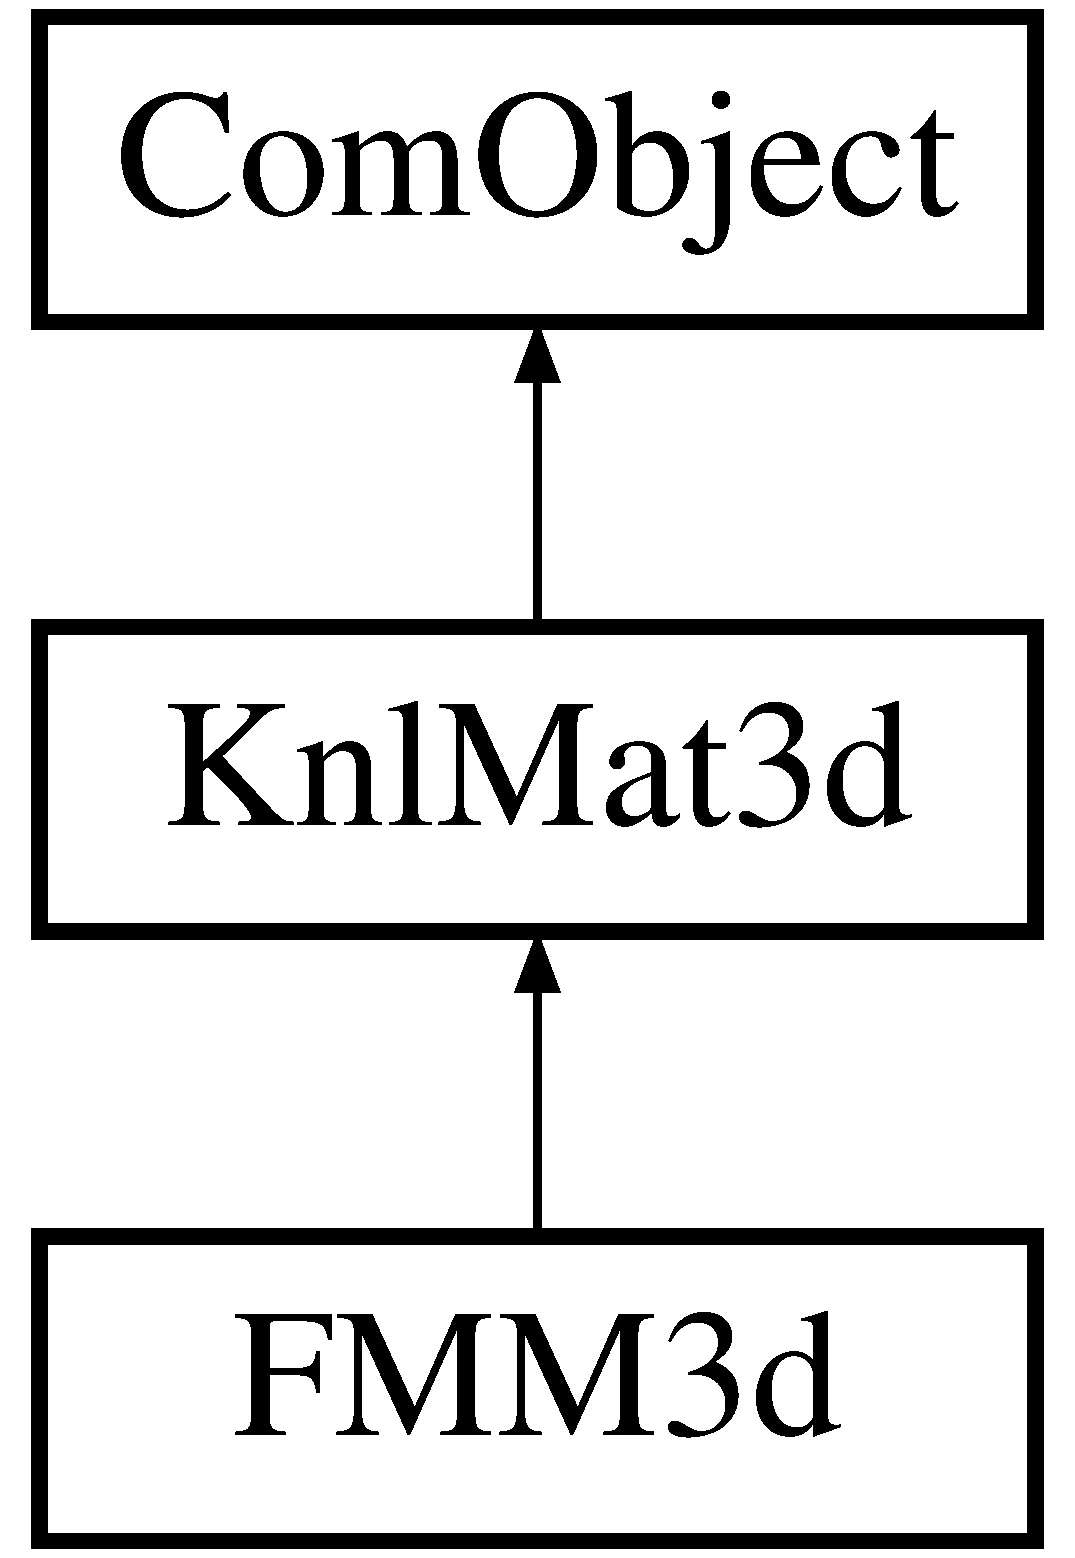
\includegraphics[height=3cm]{classFMM3d}
\end{center}
\end{figure}


\subsection{Detailed Description}
FMM3d sequential class. 

FMM3d implements {\bf Knl\-Mat3d}{\rm (p.\,\pageref{classKnlMat3d})} 



Definition at line 31 of file fmm3d.hpp.\subsection*{Public Types}
\begin{CompactItemize}
\item 
typedef pair$<$ int, int $>$ {\bf intpair}
\item 
enum \{ {\bf UE} = 0, 
{\bf UC} = 1, 
{\bf DE} = 2, 
{\bf DC} = 3
 \}
\end{CompactItemize}
\subsection*{Public Member Functions}
\begin{CompactItemize}
\item 
{\bf FMM3d} (const string \&p)
\item 
{\bf $\sim$FMM3d} ()
\item 
Point3 \& {\bf center} ()
\item 
int \& {\bf root\-Level} ()
\item 
int \& {\bf np} ()
\item 
int {\bf setup} (map$<$ string, string $>$ \&opts)
\item 
int {\bf evaluate} (const Dbl\-Num\-Vec \&src\-Den, Dbl\-Num\-Vec \&trg\-Val)
\item 
int {\bf check} (const Dbl\-Num\-Vec \&src\-Den, Dbl\-Num\-Vec \&trg\-Val, int num\-Chk, double \&relative\-Err)
\item 
{\bf Let3d} $\ast$ {\bf let} ()
\item 
{\bf Mat\-Mgnt3d} $\ast$ {\bf matmgnt} ()
\item 
vector$<$ {\bf Node} $>$ \& {\bf node\-Vec} ()
\item 
{\bf Node} \& {\bf node} (int g\-Node\-Idx)
\end{CompactItemize}
\subsection*{Protected Member Functions}
\begin{CompactItemize}
\item 
int {\bf dat\-Sze} (int tp)
\item 
int {\bf Src\-Equ2Trg\-Chk\_\-dgemv} (const Dbl\-Num\-Mat \&src\-Pos, const Dbl\-Num\-Mat \&src\-Nor, const Dbl\-Num\-Mat \&trg\-Pos, const Dbl\-Num\-Vec \&src\-Den, Dbl\-Num\-Vec \&trg\-Val)
\item 
int {\bf Src\-Equ2Upw\-Chk\_\-dgemv} (const Dbl\-Num\-Mat \&src\-Pos, const Dbl\-Num\-Mat \&src\-Nor, Point3 trg\-Ctr, double trg\-Rad, const Dbl\-Num\-Vec \&src\-Den, Dbl\-Num\-Vec \&trg\-Val)
\item 
int {\bf Src\-Equ2Dwn\-Chk\_\-dgemv} (const Dbl\-Num\-Mat \&src\-Pos, const Dbl\-Num\-Mat \&src\-Nor, Point3 trg\-Ctr, double trg\-Rad, const Dbl\-Num\-Vec \&src\-Den, Dbl\-Num\-Vec \&trg\-Val)
\item 
int {\bf Dwn\-Equ2Trg\-Chk\_\-dgemv} (Point3 src\-Ctr, double src\-Rad, const Dbl\-Num\-Mat \&trg\-Pos, const Dbl\-Num\-Vec \&src\-Den, Dbl\-Num\-Vec \&trg\-Val)
\item 
int {\bf Upw\-Equ2Trg\-Chk\_\-dgemv} (Point3 src\-Ctr, double src\-Rad, const Dbl\-Num\-Mat \&trg\-Pos, const Dbl\-Num\-Vec \&src\-Den, Dbl\-Num\-Vec \&trg\-Val)
\item 
Dbl\-Num\-Mat {\bf src\-Exa\-Pos} (int g\-Node\-Idx)
\item 
Dbl\-Num\-Mat {\bf src\-Exa\-Nor} (int g\-Node\-Idx)
\item 
Dbl\-Num\-Vec {\bf src\-Exa\-Den} (int g\-Node\-Idx)
\item 
Dbl\-Num\-Vec {\bf src\-Upw\-Equ\-Den} (int g\-Node\-Idx)
\item 
Dbl\-Num\-Vec {\bf src\-Upw\-Chk\-Val} (int g\-Node\-Idx)
\item 
Dbl\-Num\-Mat {\bf trg\-Exa\-Pos} (int g\-Node\-Idx)
\item 
Dbl\-Num\-Vec {\bf trg\-Exa\-Val} (int g\-Node\-Idx)
\item 
Dbl\-Num\-Vec {\bf trg\-Dwn\-Equ\-Den} (int g\-Node\-Idx)
\item 
Dbl\-Num\-Vec {\bf trg\-Dwn\-Chk\-Val} (int g\-Node\-Idx)
\item 
int {\bf src\-Data} ()
\item 
int {\bf trg\-Data} ()
\end{CompactItemize}
\subsection*{Protected Attributes}
\begin{CompactItemize}
\item 
Point3 {\bf \_\-center}
\item 
int {\bf \_\-root\-Level}
\item 
int {\bf \_\-np}
\item 
{\bf Let3d} $\ast$ {\bf \_\-let}
\item 
{\bf Mat\-Mgnt3d} $\ast$ {\bf \_\-matmgnt}
\item 
vector$<$ {\bf Node} $>$ {\bf \_\-node\-Vec}
\item 
Dbl\-Num\-Mat {\bf \_\-src\-Exa\-Pos}
\item 
Dbl\-Num\-Mat {\bf \_\-src\-Exa\-Nor}
\item 
Dbl\-Num\-Vec {\bf \_\-src\-Exa\-Den}
\item 
Dbl\-Num\-Vec {\bf \_\-src\-Upw\-Equ\-Den}
\item 
Dbl\-Num\-Vec {\bf \_\-src\-Upw\-Chk\-Val}
\item 
Dbl\-Num\-Mat {\bf \_\-trg\-Exa\-Pos}
\item 
Dbl\-Num\-Vec {\bf \_\-trg\-Exa\-Val}
\item 
Dbl\-Num\-Vec {\bf \_\-trg\-Dwn\-Equ\-Den}
\item 
Dbl\-Num\-Vec {\bf \_\-trg\-Dwn\-Chk\-Val}
\item 
{\bf Kernel3d} {\bf \_\-knl\_\-mm}
\item 
int {\bf \_\-mul\_\-mm}
\end{CompactItemize}
\subsection*{Classes}
\begin{CompactItemize}
\item 
class {\bf Node}
\begin{CompactList}\small\item\em {\bf Node}{\rm (p.\,\pageref{classFMM3d_1_1Node})} Class for {\bf FMM3d}{\rm (p.\,\pageref{classFMM3d})}. \item\end{CompactList}\end{CompactItemize}


\subsection{Member Typedef Documentation}
\index{FMM3d@{FMM3d}!intpair@{intpair}}
\index{intpair@{intpair}!FMM3d@{FMM3d}}
\subsubsection{\setlength{\rightskip}{0pt plus 5cm}typedef pair$<$int,int$>$ {\bf FMM3d::intpair}}\label{classFMM3d_516fcca2e14cd2e14fd71db54824f696_516fcca2e14cd2e14fd71db54824f696}




Definition at line 34 of file fmm3d.hpp.

\subsection{Member Enumeration Documentation}
\subsubsection{\setlength{\rightskip}{0pt plus 5cm}anonymous enum}\label{classFMM3d_dca29a1140aadadfd92b34a02fa516ef_dca29a1140aadadfd92b34a02fa516ef}


UE = Upper Equivalent UC = Upper Check DE = Downward Equivalent DC = Downward Check \begin{Desc}
\item[Enumerator: ]\par
\begin{description}
\index{UE@{UE}!FMM3d@{FMM3d}}\index{FMM3d@{FMM3d}!UE@{UE}}\item[{\em 
UE\label{classFMM3d_dca29a1140aadadfd92b34a02fa516ef_dca29a1140aadadfd92b34a02fa516ef0612e93d65abcdaeed533a0876474251}
}]\index{UC@{UC}!FMM3d@{FMM3d}}\index{FMM3d@{FMM3d}!UC@{UC}}\item[{\em 
UC\label{classFMM3d_dca29a1140aadadfd92b34a02fa516ef_dca29a1140aadadfd92b34a02fa516ef6a2fb30a2dacdda4d74122697262a8b7}
}]\index{DE@{DE}!FMM3d@{FMM3d}}\index{FMM3d@{FMM3d}!DE@{DE}}\item[{\em 
DE\label{classFMM3d_dca29a1140aadadfd92b34a02fa516ef_dca29a1140aadadfd92b34a02fa516ef3a52f3c22ed6fcde5bf696a6c02c9e73}
}]\index{DC@{DC}!FMM3d@{FMM3d}}\index{FMM3d@{FMM3d}!DC@{DC}}\item[{\em 
DC\label{classFMM3d_dca29a1140aadadfd92b34a02fa516ef_dca29a1140aadadfd92b34a02fa516efcf75e54791dd1f49f918345fdfe2430b}
}]\end{description}
\end{Desc}



Definition at line 40 of file fmm3d.hpp.

\footnotesize\begin{verbatim}40 {        UE=0,   UC=1,   DE=2,   DC=3,  };
\end{verbatim}\normalsize 




\subsection{Constructor \& Destructor Documentation}
\index{FMM3d@{FMM3d}!FMM3d@{FMM3d}}
\index{FMM3d@{FMM3d}!FMM3d@{FMM3d}}
\subsubsection{\setlength{\rightskip}{0pt plus 5cm}FMM3d::FMM3d (const string \& {\em p})}\label{classFMM3d_c6779767af55d215c788dcaf4dfbaf6e_c6779767af55d215c788dcaf4dfbaf6e}




Definition at line 23 of file fmm3d.cpp.

\footnotesize\begin{verbatim}23                            :
24   KnlMat3d(p), _center(0,0,0), _rootLevel(0),
25   _np(6), _let(NULL), _matmgnt(NULL)
26 {
27 }

\end{verbatim}\normalsize 


\index{FMM3d@{FMM3d}!~FMM3d@{$\sim$FMM3d}}
\index{~FMM3d@{$\sim$FMM3d}!FMM3d@{FMM3d}}
\subsubsection{\setlength{\rightskip}{0pt plus 5cm}FMM3d::$\sim$FMM3d ()}\label{classFMM3d_95ad154aae7c25cde0cc2a7108470c36_95ad154aae7c25cde0cc2a7108470c36}




Definition at line 29 of file fmm3d.cpp.

References \_\-let.

\footnotesize\begin{verbatim}30 {
31   if(_let!=NULL)         delete _let;
32 }
\end{verbatim}\normalsize 




\subsection{Member Function Documentation}
\index{FMM3d@{FMM3d}!center@{center}}
\index{center@{center}!FMM3d@{FMM3d}}
\subsubsection{\setlength{\rightskip}{0pt plus 5cm}Point3\& FMM3d::center ()\hspace{0.3cm}{\tt  [inline]}}\label{classFMM3d_5c0517b22b09f08712cbfd01aa1f29d7_5c0517b22b09f08712cbfd01aa1f29d7}


Return center of toplevel box 

Definition at line 109 of file fmm3d.hpp.

References \_\-center.

\footnotesize\begin{verbatim}109 { return _center; }
\end{verbatim}\normalsize 


\index{FMM3d@{FMM3d}!check@{check}}
\index{check@{check}!FMM3d@{FMM3d}}
\subsubsection{\setlength{\rightskip}{0pt plus 5cm}int FMM3d::check (const Dbl\-Num\-Vec \& {\em src\-Den}, Dbl\-Num\-Vec \& {\em trg\-Val}, int {\em num\-Chk}, double \& {\em relative\-Err})}\label{classFMM3d_03ae26a8343213f8e305ed8df685173f_03ae26a8343213f8e305ed8df685173f}


Check relative error - in fmm\_\-check.cpp 

Definition at line 25 of file fmm3d\_\-check.cpp.

References Knl\-Mat3d::\_\-src\-Pos, Knl\-Mat3d::\_\-trg\-Pos, Knl\-Mat3d::dim(), Knl\-Mat3d::src\-DOF(), and Knl\-Mat3d::trg\-DOF().

\footnotesize\begin{verbatim}26 {
27   iA(_trgPos->n()>0); //have things to check
28   int dim = this->dim();
29   int srcDOF = this->srcDOF();
30   int trgDOF = this->trgDOF();
31   int srcNum = _srcPos->n();
32   int trgNum = _trgPos->n();   //int lclnum = this->lclnum();
33   
34   //1. select point to check
35   vector<int> chkVec(numChk);
36   for(int k=0; k<numChk; k++) {
37          chkVec[k] = int( floor(drand48()*trgNum) );     iA(chkVec[k]>=0 && chkVec[k]<trgNum);
38   }
39   DblNumMat ChkPos(dim, numChk);
40   DblNumVec chkVal(numChk*trgDOF);
41   DblNumVec chkDen(numChk*trgDOF);
42   for(int k=0; k<numChk; k++) {
43          for(int i=0; i<dim; i++)               ChkPos(i, k) = (*_trgPos)(i, chkVec[k]);
44          for(int i=0; i<trgDOF;i++)             chkVal(k*trgDOF+i) = trgVal(chkVec[k]*trgDOF+i);
45   }
46   
47   //2. compute and gather
48   DblNumMat inter(trgDOF, srcNum*srcDOF);
49   for(int i=0; i<numChk; i++) {
50          DblNumMat oneChkPos(dim, 1, false, ChkPos.clmdata(i));
51          DblNumVec onechkDen(trgDOF, false, chkDen.data()+i*trgDOF);
52          iC( _knl.kernel(*_srcPos, *_srcNor, oneChkPos, inter) );
53          iC( dgemv(1.0, inter, srcden, 0.0, onechkDen) );
54   }
55   
56   //3. distribute to individual
57   for(int k=0; k<numChk; k++)
58          for(int i=0; i<trgDOF; i++)
59                 chkDen(k*trgDOF+i) -= chkVal(k*trgDOF+i);
60   
61   double vn = 0;  double en = 0;
62   for(int k=0; k<numChk; k++)
63          for(int i=0; i<trgDOF; i++) {
64                 vn += chkVal(k*trgDOF+i) * chkVal(k*trgDOF+i);
65                 en += chkDen(k*trgDOF+i) * chkDen(k*trgDOF+i);
66          }
67   vn = sqrt(vn);
68   en = sqrt(en);
69   
70   //cerr<<"relative error: "<<en/vn<<endl;  cerr<<"error norm    : "<<en<<endl;  cerr<<"solution norm : "<<vn<<endl;
71   rerr = en/vn; //relative error
72   
73   return 0;
74 }
\end{verbatim}\normalsize 


\index{FMM3d@{FMM3d}!datSze@{datSze}}
\index{datSze@{datSze}!FMM3d@{FMM3d}}
\subsubsection{\setlength{\rightskip}{0pt plus 5cm}int FMM3d::dat\-Sze (int {\em tp})\hspace{0.3cm}{\tt  [inline, protected]}}\label{classFMM3d_e698f5e6e784c12d19a62b0d40456fc6_e698f5e6e784c12d19a62b0d40456fc6}


Data Size 

Definition at line 128 of file fmm3d.hpp.

References \_\-matmgnt, and Mat\-Mgnt3d::pln\-Dat\-Sze().

Referenced by src\-Data(), src\-Upw\-Chk\-Val(), src\-Upw\-Equ\-Den(), trg\-Data(), trg\-Dwn\-Chk\-Val(), and trg\-Dwn\-Equ\-Den().

\footnotesize\begin{verbatim}128 { return _matmgnt->plnDatSze(tp); }
\end{verbatim}\normalsize 


\index{FMM3d@{FMM3d}!DwnEqu2TrgChk_dgemv@{DwnEqu2TrgChk\_\-dgemv}}
\index{DwnEqu2TrgChk_dgemv@{DwnEqu2TrgChk\_\-dgemv}!FMM3d@{FMM3d}}
\subsubsection{\setlength{\rightskip}{0pt plus 5cm}int FMM3d::Dwn\-Equ2Trg\-Chk\_\-dgemv (Point3 {\em src\-Ctr}, double {\em src\-Rad}, const Dbl\-Num\-Mat \& {\em trg\-Pos}, const Dbl\-Num\-Vec \& {\em src\-Den}, Dbl\-Num\-Vec \& {\em trg\-Val})\hspace{0.3cm}{\tt  [protected]}}\label{classFMM3d_044a9a8966c365ba77585ecc38a2073e_044a9a8966c365ba77585ecc38a2073e}


Downward Equivalent To Target Check 

Definition at line 84 of file fmm3d.cpp.

References \_\-knl\_\-mm, \_\-matmgnt, DE, Kernel3d::kernel(), Mat\-Mgnt3d::local\-Pos(), Kernel3d::src\-DOF(), and Kernel3d::trg\-DOF().

\footnotesize\begin{verbatim}85 {
86   int TMAX = 1024;
87   if(trgPos.n()<=TMAX) {
88          DblNumMat srcPos; iC( _matmgnt->localPos(DE, srcCtr, srcRad, srcPos) );
89          int M = trgPos.n() * _knl_mm.trgDOF();
90          int N = srcPos.n() * _knl_mm.srcDOF();
91          DblNumMat tmp(M,N);
92          iC( _knl_mm.kernel(srcPos, srcPos, trgPos, tmp) );
93          iC( dgemv(1.0, tmp, srcDen, 1.0, trgVal) );
94   } else {
95          DblNumMat srcPos; iC( _matmgnt->localPos(DE, srcCtr, srcRad, srcPos) );
96          int RUNS = (trgPos.n()-1) / TMAX + 1;
97          for(int r=0; r<RUNS; r++) {
98                 int stt = r*TMAX;
99                 int end = min((r+1)*TMAX, trgPos.n());
100                 int num = end-stt;
101                 int M = num * _knl_mm.trgDOF();
102                 int N = srcPos.n() * _knl_mm.srcDOF();
103                 DblNumMat tps(dim(), num, false, trgPos.data() + stt*dim());
104                 DblNumVec tvl(num*_knl_mm.trgDOF(), false, trgVal.data() + stt*_knl_mm.trgDOF());
105                 DblNumMat tmp(M, N);
106                 iC( _knl_mm.kernel(srcPos, srcPos, tps, tmp) );
107                 iC( dgemv(1.0, tmp, srcDen, 1.0, tvl) );
108          }
109   }
110   return 0;
111 }
\end{verbatim}\normalsize 


\index{FMM3d@{FMM3d}!evaluate@{evaluate}}
\index{evaluate@{evaluate}!FMM3d@{FMM3d}}
\subsubsection{\setlength{\rightskip}{0pt plus 5cm}int FMM3d::evaluate (const Dbl\-Num\-Vec \& {\em src\-Den}, Dbl\-Num\-Vec \& {\em trg\-Val})\hspace{0.3cm}{\tt  [virtual]}}\label{classFMM3d_3d2ce8cfb3d9632d6b69352f1bb5eda2_3d2ce8cfb3d9632d6b69352f1bb5eda2}


Evaluate - in {\bf fmm3d\_\-eval.cpp}{\rm (p.\,\pageref{fmm3d__eval_8cpp})} 

Implements {\bf Knl\-Mat3d} {\rm (p.\,\pageref{classKnlMat3d_fcf3de1e6ce4ee024ef0d320363bd920_fcf3de1e6ce4ee024ef0d320363bd920})}.

Definition at line 25 of file fmm3d\_\-eval.cpp.

References \_\-let, \_\-matmgnt, \_\-src\-Exa\-Den, \_\-src\-Upw\-Chk\-Val, \_\-src\-Upw\-Equ\-Den, \_\-trg\-Dwn\-Chk\-Val, \_\-trg\-Dwn\-Equ\-Den, \_\-trg\-Exa\-Val, LET\_\-SRCNODE, Let3d::node(), Mat\-Mgnt3d::report(), Knl\-Mat3d::src\-DOF(), src\-Exa\-Den(), Let3d::tag(), Let3d::terminal(), Knl\-Mat3d::trg\-DOF(), and Let3d::upw\-Order\-Collect().

\footnotesize\begin{verbatim}26 {
27   _matmgnt->report();
28   //-----------------------------------
29   iA(srcDen.m()==srcDOF()*(*_srcPos).n());  iA(trgVal.m()==trgDOF()*(*_trgPos).n());
30   
31   //cerr<<"fmm src and trg numbers "<<pglbnum(_srcPos)<<" "<<pglbnum(_trgPos)<<endl;
32   int srcDOF = this->srcDOF();
33   int trgDOF = this->trgDOF();
34   
35   //1. zero out Vecs
36   setvalue(trgVal, 0.0);
37   
38   setvalue(_srcExaDen, 0.0);
39   setvalue(_srcUpwEquDen, 0.0);
40   setvalue(_srcUpwChkVal, 0.0);
41   
42   setvalue(_trgExaVal, 0.0);
43   setvalue(_trgDwnEquDen, 0.0);
44   setvalue(_trgDwnChkVal, 0.0);
45   clock_t ck0, ck1;
46   //CLOCKING;
47   ck0 = clock();
48   vector<int> ordVec; iC( _let->upwOrderCollect(ordVec) ); //BOTTOM UP
49 
50   //2. for cbtr, load ExaDen
51   ck0 = clock();
52   for(int i=0; i<ordVec.size(); i++) {
53          int gNodeIdx = ordVec[i];
54          if(_let->tag(gNodeIdx) & LET_SRCNODE) {
55                 if(_let->terminal(gNodeIdx)==true) {
56                   DblNumVec srcExaDen(this->srcExaDen(gNodeIdx));
57                   vector<int>& curVecIdxs = _let->node(gNodeIdx).srcOwnVecIdxs();
58                   for(int k=0; k<curVecIdxs.size(); k++) {
59                          int poff = curVecIdxs[k];
60                          for(int d=0; d<srcDOF; d++) {
61                                 srcExaDen(k*srcDOF+d) = srcDen(poff*srcDOF+d);
62                          }
63                   }
64                 }
65          }
66   }
67   //ck1 = clock();  cerr<<"load  "<<double(ck1-ck0)/CLOCKS_PER_SEC<<endl;  
68   
69   //3. up computation
70   ck0 = clock();
71   for(int i=0; i<ordVec.size(); i++) {
72          int gNodeIdx = ordVec[i];
73          if(_let->tag(gNodeIdx) & LET_SRCNODE) {                //GNTra gnt = _let->gNodeIdx2gnt(gNodeIdx);
74                 //if(_let->depth(gNodeIdx)>=2) {
75                 if(_let->depth(gNodeIdx)>=0) {
76                   DblNumVec srcUpwChkValgNodeIdx(srcUpwChkVal(gNodeIdx));
77                   DblNumVec srcUpwEquDengNodeIdx(srcUpwEquDen(gNodeIdx));
78                   if(_let->terminal(gNodeIdx)==true) {
79                          //S2M - Source -> Multipole Exapnsion
80                          iC( SrcEqu2UpwChk_dgemv(srcExaPos(gNodeIdx), srcExaNor(gNodeIdx), _let->center(gNodeIdx), _let->radius(gNodeIdx), srcExaDen(gNodeIdx), srcUpwChkValgNodeIdx) );
81                   } else {
82                          //M2M - Multipole -> Multipole
83                          for(int a=0; a<2; a++) {
84                                 for(int b=0; b<2; b++) {
85                                   for(int c=0; c<2; c++) {
86                                          Index3 idx(a,b,c);
87                                          int chi = _let->child(gNodeIdx, idx);
88                                          if(_let->tag(chi) & LET_SRCNODE) {
89                                                 iC( _matmgnt->UpwEqu2UpwChk_dgemv(_let->depth(chi)+_rootLevel, idx, srcUpwEquDen(chi), srcUpwChkValgNodeIdx) );
90                                          }
91                                   }
92                                 }
93                          }
94                   }
95                   //M2M - Multipole -> Multipole
96                   iC( _matmgnt->UpwChk2UpwEqu_dgemv(_let->depth(gNodeIdx)+_rootLevel, srcUpwChkValgNodeIdx, srcUpwEquDengNodeIdx) );
97                 }
98          }
99   }
100   ordVec.clear();  iC( _let->dwnOrderCollect(ordVec) );
101   //U - list contribution calculation
102   ck0 = clock();
103   for(int i=0; i<ordVec.size(); i++) {
104          int gNodeIdx = ordVec[i];
105          if(_let->tag(gNodeIdx) & LET_TRGNODE) { //evaluator
106                 if( _let->terminal(gNodeIdx)==true ) { //terminal       
107                   Let3d::Node& curNode = _let->node(gNodeIdx);
108                   DblNumVec trgExaValgNodeIdx(trgExaVal(gNodeIdx));
109                   DblNumMat trgExaPosgNodeIdx(trgExaPos(gNodeIdx));
110                   for(vector<int>::iterator vi=curNode.Unodes().begin(); vi!=curNode.Unodes().end(); vi++) {
111                          //S2T - source -> target
112                          iC( SrcEqu2TrgChk_dgemv(srcExaPos(*vi), srcExaNor(*vi), trgExaPosgNodeIdx, srcExaDen(*vi), trgExaValgNodeIdx) );
113                   }
114                 }
115          }
116   }
117   //V - list contribution calculation
118   ck0 = clock();
119   for(int i=0; i<ordVec.size(); i++) {
120          int gNodeIdx = ordVec[i];
121          if( _let->tag(gNodeIdx) & LET_TRGNODE) { //eValuator           //GNTra gnt = _let->gNodeIdx2gnt(gNodeIdx);
122                 Point3 gNodeIdxCtr(_let->center(gNodeIdx));
123                 double D = 2.0 * _let->radius(gNodeIdx);
124                 DblNumVec trgDwnChkVal(this->trgDwnChkVal(gNodeIdx));
125                 Let3d::Node& curNode = _let->node(gNodeIdx);
126                 for(vector<int>::iterator vi=curNode.Vnodes().begin(); vi!=curNode.Vnodes().end(); vi++) {
127                   Point3 viCtr(_let->center(*vi));
128                   Index3 idx;
129                   for(int d=0; d<dim(); d++){
130                          idx(d) = int(round( (viCtr[d]-gNodeIdxCtr[d])/D ));
131                   }
132                   Node& srcPtr = node(*vi);
133                   Node& trgPtr = node(gNodeIdx);
134                   if(srcPtr.VotCnt()==0) {
135                          srcPtr.effDen().resize( _matmgnt->effDatSze(UE) );                      setvalue(srcPtr.effDen(), 0.0);//1. resize effDen
136                          iC( _matmgnt->plnDen2EffDen(_let->depth(gNodeIdx)+_rootLevel, srcUpwEquDen(*vi),  srcPtr.effDen()) );                   //2. transform from upeDen to effDen
137                   }
138                   if(trgPtr.VinCnt()==0) {
139                          trgPtr.effVal().resize( _matmgnt->effDatSze(DC) );                      setvalue(trgPtr.effVal(), 0.0);                         //1. resize effVal
140                   }
141                   //M2L - multipole -> local
142                   iC( _matmgnt->UpwEqu2DwnChk_dgemv(_let->depth(gNodeIdx)+_rootLevel, idx, srcPtr.effDen(), trgPtr.effVal()) );
143                   
144                   srcPtr.VotCnt()++;
145                   trgPtr.VinCnt()++;
146                   if(srcPtr.VotCnt()==srcPtr.VotNum()) {
147                          srcPtr.effDen().resize(0);                      //1. resize effDen to 0
148                          srcPtr.VotCnt()=0;
149                   }
150                   if(trgPtr.VinCnt()==trgPtr.VinNum()) {
151                          iC( _matmgnt->effVal2PlnVal(_let->depth(gNodeIdx)+_rootLevel, trgPtr.effVal(), trgDwnChkVal) );                         //1. transform from effVal to dncVal
152                          trgPtr.effVal().resize(0); //2. resize effVal to 0
153                          trgPtr.VinCnt()=0;
154                   }
155                 }
156          }
157   }
158   //W - list contrubtion calculation
159   ck0 = clock();
160   for(int i=0; i<ordVec.size(); i++) {
161          int gNodeIdx = ordVec[i];
162          if( _let->tag(gNodeIdx) & LET_TRGNODE ) {
163                 if( _let->terminal(gNodeIdx)==true ) {
164                   DblNumVec trgExaVal_gNodeIdx(this->trgExaVal(gNodeIdx));
165                   Let3d::Node& curNode = _let->node(gNodeIdx);
166                   for(vector<int>::iterator vi=curNode.Wnodes().begin(); vi!=curNode.Wnodes().end(); vi++) {
167                          if(_let->terminal(*vi) && _let->node(*vi).srcExaNum()*srcDOF<_matmgnt->plnDatSze(UE)) { //use Exa instead
168                                 //S2T - source -> target
169                                 iC( SrcEqu2TrgChk_dgemv(srcExaPos(*vi), srcExaNor(*vi), trgExaPos(gNodeIdx), srcExaDen(*vi), trgExaVal_gNodeIdx) );
170                          } else {
171                                 //M2T - multipole -> target
172                                 int vni = *vi;                          
173                                 iC( UpwEqu2TrgChk_dgemv(_let->center(vni), _let->radius(vni), trgExaPos(gNodeIdx), srcUpwEquDen(*vi), trgExaVal_gNodeIdx) );
174                          }
175                   }
176                 }
177          }
178   }
179   //X - list contrubtion calculation
180   ck0 = clock();
181   for(int i=0; i<ordVec.size(); i++) {
182          int gNodeIdx = ordVec[i];
183          if( _let->tag(gNodeIdx) & LET_TRGNODE) {       
184                 Let3d::Node& curNode = _let->node(gNodeIdx);
185                 DblNumVec trgExaVal_gNodeIdx(trgExaVal(gNodeIdx));
186                 DblNumVec trgDwnChkVal_gNodeIdx(trgDwnChkVal(gNodeIdx));
187                 for(vector<int>::iterator vi=curNode.Xnodes().begin(); vi!=curNode.Xnodes().end(); vi++) {
188                   if(_let->terminal(gNodeIdx) && _let->node(gNodeIdx).trgExaNum()*trgDOF<_matmgnt->plnDatSze(DC)) { //use Exa instead
189                          iC( SrcEqu2TrgChk_dgemv(srcExaPos(*vi), srcExaNor(*vi), trgExaPos(gNodeIdx), srcExaDen(*vi), trgExaVal_gNodeIdx) );
190                   } else {
191                          //S2L - source -> local
192                          iC( SrcEqu2DwnChk_dgemv(srcExaPos(*vi), srcExaNor(*vi), _let->center(gNodeIdx), _let->radius(gNodeIdx), srcExaDen(*vi), trgDwnChkVal_gNodeIdx) );
193                   }
194                 }
195          }
196   }
197   //7. combine
198   ck0 = clock();
199   for(int i=0; i<ordVec.size(); i++) {
200          int gNodeIdx = ordVec[i];
201          if( _let->tag(gNodeIdx) & LET_TRGNODE ) { //eValuator          
202                 if(_let->depth(gNodeIdx)>=3) {
203                   int pargNodeIdx = _let->parent(gNodeIdx);     
204                   Index3 chdIdx( _let->path2Node(gNodeIdx)-2 * _let->path2Node(pargNodeIdx) );
205                   //L2L - local -> local
206                   DblNumVec trgDwnChkVal_gNodeIdx(trgDwnChkVal(gNodeIdx));
207                   iC( _matmgnt->DwnEqu2DwnChk_dgemv(_let->depth(pargNodeIdx)+_rootLevel, chdIdx, trgDwnEquDen(pargNodeIdx), trgDwnChkVal_gNodeIdx) );
208                 }
209                 if(_let->depth(gNodeIdx)>=2) {
210                   //L2L - local -> local
211                   DblNumVec trgDwnEquDen_gNodeIdx(trgDwnEquDen(gNodeIdx));
212                   iC( _matmgnt->DwnChk2DwnEqu_dgemv(_let->depth(gNodeIdx)+_rootLevel, trgDwnChkVal(gNodeIdx), trgDwnEquDen_gNodeIdx) );
213                 }
214                 if(_let->terminal(gNodeIdx)) {
215                   //L2T - local -> target
216                   DblNumVec trgExaVal_gNodeIdx(trgExaVal(gNodeIdx));
217                   iC( DwnEqu2TrgChk_dgemv(_let->center(gNodeIdx), _let->radius(gNodeIdx), trgExaPos(gNodeIdx), trgDwnEquDen(gNodeIdx), trgExaVal_gNodeIdx) );
218                 }
219          }
220   }
221   
222   //8. save trgExaVal
223   ck0 = clock();
224   for(int i=0; i<ordVec.size(); i++) {
225          int gNodeIdx = ordVec[i];
226          if( _let->tag(gNodeIdx) & LET_TRGNODE ) {
227                 if( _let->terminal(gNodeIdx)==true ) {
228                   DblNumVec trgExaVal(this->trgExaVal(gNodeIdx));
229                   vector<int>& curVecIdxs = _let->node(gNodeIdx).trgOwnVecIdxs();
230                   for(int k=0; k<curVecIdxs.size(); k++) {
231                          int poff = curVecIdxs[k];
232                          for(int d=0; d<trgDOF; d++) {
233                                 trgVal(poff*trgDOF+d) = trgExaVal(k*trgDOF+d);
234                          }
235                   }
236                 }
237          }
238   }
239   return (0);
240 }
\end{verbatim}\normalsize 


\index{FMM3d@{FMM3d}!let@{let}}
\index{let@{let}!FMM3d@{FMM3d}}
\subsubsection{\setlength{\rightskip}{0pt plus 5cm}{\bf Let3d}$\ast$ FMM3d::let ()\hspace{0.3cm}{\tt  [inline]}}\label{classFMM3d_ab08876abdb0f42b280939bc45a41dad_ab08876abdb0f42b280939bc45a41dad}




Definition at line 121 of file fmm3d.hpp.

References \_\-let.

\footnotesize\begin{verbatim}121 { return _let; }
\end{verbatim}\normalsize 


\index{FMM3d@{FMM3d}!matmgnt@{matmgnt}}
\index{matmgnt@{matmgnt}!FMM3d@{FMM3d}}
\subsubsection{\setlength{\rightskip}{0pt plus 5cm}{\bf Mat\-Mgnt3d}$\ast$ FMM3d::matmgnt ()\hspace{0.3cm}{\tt  [inline]}}\label{classFMM3d_eb0e3260b02ea4bd6f7a2303874f53bf_eb0e3260b02ea4bd6f7a2303874f53bf}




Definition at line 122 of file fmm3d.hpp.

References \_\-matmgnt.

\footnotesize\begin{verbatim}122 { return _matmgnt; }
\end{verbatim}\normalsize 


\index{FMM3d@{FMM3d}!node@{node}}
\index{node@{node}!FMM3d@{FMM3d}}
\subsubsection{\setlength{\rightskip}{0pt plus 5cm}{\bf Node}\& FMM3d::node (int {\em g\-Node\-Idx})\hspace{0.3cm}{\tt  [inline]}}\label{classFMM3d_f259ccf218dbf0a04530841785f1a8b0_f259ccf218dbf0a04530841785f1a8b0}




Definition at line 124 of file fmm3d.hpp.

References \_\-node\-Vec.

Referenced by src\-Exa\-Pos().

\footnotesize\begin{verbatim}124 { return _nodeVec[gNodeIdx]; }
\end{verbatim}\normalsize 


\index{FMM3d@{FMM3d}!nodeVec@{nodeVec}}
\index{nodeVec@{nodeVec}!FMM3d@{FMM3d}}
\subsubsection{\setlength{\rightskip}{0pt plus 5cm}vector$<${\bf Node}$>$\& FMM3d::node\-Vec ()\hspace{0.3cm}{\tt  [inline]}}\label{classFMM3d_44c0c8da466878274feb4ce060c10b9b_44c0c8da466878274feb4ce060c10b9b}




Definition at line 123 of file fmm3d.hpp.

References \_\-node\-Vec.

\footnotesize\begin{verbatim}123 { return _nodeVec; }
\end{verbatim}\normalsize 


\index{FMM3d@{FMM3d}!np@{np}}
\index{np@{np}!FMM3d@{FMM3d}}
\subsubsection{\setlength{\rightskip}{0pt plus 5cm}int\& FMM3d::np ()\hspace{0.3cm}{\tt  [inline]}}\label{classFMM3d_79545716c1fbc95cbd811a65ffa9f767_79545716c1fbc95cbd811a65ffa9f767}




Definition at line 112 of file fmm3d.hpp.

References \_\-np.

\footnotesize\begin{verbatim}112 { return _np; }  
\end{verbatim}\normalsize 


\index{FMM3d@{FMM3d}!rootLevel@{rootLevel}}
\index{rootLevel@{rootLevel}!FMM3d@{FMM3d}}
\subsubsection{\setlength{\rightskip}{0pt plus 5cm}int\& FMM3d::root\-Level ()\hspace{0.3cm}{\tt  [inline]}}\label{classFMM3d_f80fcb36cb42936f1912fe8c85ec96e4_f80fcb36cb42936f1912fe8c85ec96e4}


Return the rootlevel. 2$^\wedge$(-rootlvl) is the radius of the toplevel box 

Definition at line 111 of file fmm3d.hpp.

References \_\-root\-Level.

\footnotesize\begin{verbatim}111 { return _rootLevel; }
\end{verbatim}\normalsize 


\index{FMM3d@{FMM3d}!setup@{setup}}
\index{setup@{setup}!FMM3d@{FMM3d}}
\subsubsection{\setlength{\rightskip}{0pt plus 5cm}int FMM3d::setup (map$<$ string, string $>$ \& {\em opts})\hspace{0.3cm}{\tt  [virtual]}}\label{classFMM3d_d134e155a30bcbea9ad038ffcd737ddc_d134e155a30bcbea9ad038ffcd737ddc}


Setup function 

Implements {\bf Knl\-Mat3d} {\rm (p.\,\pageref{classKnlMat3d_24cbbecf677cd909a522d252feebf2c6_24cbbecf677cd909a522d252feebf2c6})}.

Definition at line 26 of file fmm3d\_\-setup.cpp.

References \_\-np, and Com\-Object::prefix().

\footnotesize\begin{verbatim}27 {
28   //-----------------------------------------------------
29   map<string,string>::iterator mi;
30   mi = opts.find("-" + prefix() + "np"); iA(mi!=opts.end());
31   { istringstream ss((*mi).second); ss>>_np; }
32     
33   //-----------------------------------------------------
34   iA(_srcPos!=NULL && _srcNor!=NULL && _trgPos!=NULL);
35   iA((*_srcPos).m()==dim() && (*_trgPos).m()==dim());  //nothing to do
36   //1. _let
37   _let = new Let3d(prefix()+"let3d_");
38   _let->srcPos()=_srcPos;  _let->trgPos()=_trgPos;  _let->center()=_center;  _let->rootLevel()=_rootLevel;
39   iC( _let->setup(opts) );
40   //2. decide _eq_mm and _mul_mm, and get matmgnt based on that
41   switch(_knl.kernelType()) {
42          //laplace kernels
43   case KNL_LAP_S_U: _knl_mm = Kernel3d(KNL_LAP_S_U, _knl.coefs()); break;
44   case KNL_LAP_D_U: _knl_mm = Kernel3d(KNL_LAP_S_U, _knl.coefs()); break;
45          //stokes kernels
46   case KNL_STK_S_U: _knl_mm = Kernel3d(KNL_STK_F_U, _knl.coefs()); break;
47   case KNL_STK_S_P: _knl_mm = Kernel3d(KNL_LAP_S_U, vector<double>()); break;
48   case KNL_STK_D_U: _knl_mm = Kernel3d(KNL_STK_F_U, _knl.coefs()); break;
49   case KNL_STK_D_P: _knl_mm = Kernel3d(KNL_LAP_S_U, vector<double>()); break;
50          //navier kernels
51   case KNL_NAV_S_U: _knl_mm = Kernel3d(KNL_NAV_S_U, _knl.coefs()); break;
52   case KNL_NAV_D_U: _knl_mm = Kernel3d(KNL_NAV_S_U, _knl.coefs()); break;
53          //others
54   case KNL_SQRTLAP: _knl_mm = Kernel3d(KNL_SQRTLAP, _knl.coefs()); break;
55   case KNL_EXP    : _knl_mm = Kernel3d(KNL_EXP    , _knl.coefs()); break;
56   default: iA(0);
57   }
58   _mul_mm = 1; //for the time being
59   
60   _matmgnt  = MatMgnt3d::getmmptr(_knl_mm, _np);
61   //3. self setup
62   iC( srcData() );
63   iC( trgData() );
64   //-----------------------------------------------------
65   return (0);
66 }
\end{verbatim}\normalsize 


\index{FMM3d@{FMM3d}!srcData@{srcData}}
\index{srcData@{srcData}!FMM3d@{FMM3d}}
\subsubsection{\setlength{\rightskip}{0pt plus 5cm}int FMM3d::src\-Data ()\hspace{0.3cm}{\tt  [protected]}}\label{classFMM3d_44ef9057a3adc0372c2569c172064dac_44ef9057a3adc0372c2569c172064dac}


return source data 

Definition at line 68 of file fmm3d\_\-setup.cpp.

References \_\-let, \_\-src\-Exa\-Den, \_\-src\-Exa\-Nor, \_\-src\-Exa\-Pos, \_\-src\-Upw\-Chk\-Val, \_\-src\-Upw\-Equ\-Den, dat\-Sze(), Knl\-Mat3d::dim(), LET\_\-SRCNODE, Let3d::node(), Knl\-Mat3d::src\-DOF(), Let3d::src\-Exa\-Cnt(), src\-Exa\-Nor(), src\-Exa\-Pos(), Let3d::src\-Node\-Cnt(), Let3d::tag(), Let3d::terminal(), UC, UE, and Let3d::upw\-Order\-Collect().

\footnotesize\begin{verbatim}69 {
70   //1. create vecs
71   int srcNodeCnt = _let->srcNodeCnt();
72   int srcExaCnt = _let->srcExaCnt();
73   _srcExaPos.resize(dim(), srcExaCnt);
74   _srcExaNor.resize(dim(), srcExaCnt);
75   _srcExaDen.resize(srcExaCnt * srcDOF());
76   _srcUpwEquDen.resize(srcNodeCnt * datSze(UE));
77   _srcUpwChkVal.resize(srcNodeCnt * datSze(UC));
78   
79   //2. gather the Position using the Pos scatter
80   vector<int> ordVec;  iC( _let->upwOrderCollect(ordVec) );
81   for(int i=0; i<ordVec.size(); i++) {
82          int gNodeIdx = ordVec[i];
83          if(_let->tag(gNodeIdx) & LET_SRCNODE) { //contributor
84                 if(_let->terminal(gNodeIdx)==true) { //terminal cbtr
85                   DblNumMat srcExaPos(this->srcExaPos(gNodeIdx));
86                   DblNumMat srcExaNor(this->srcExaNor(gNodeIdx));
87                   vector<int>& curVecIdxs = _let->node(gNodeIdx).srcOwnVecIdxs();
88                   for(int k=0; k < curVecIdxs.size(); k++) {
89                          int poff = curVecIdxs[k];
90                          for(int d=0; d < dim(); d++) {
91                                 srcExaPos(d,k) = (*_srcPos)(d,poff);//Pos
92                                 srcExaNor(d,k) = (*_srcNor)(d,poff);//Nor
93                          }
94                   }
95                 }
96          }
97   }
98   return (0);
99 }
\end{verbatim}\normalsize 


\index{FMM3d@{FMM3d}!SrcEqu2DwnChk_dgemv@{SrcEqu2DwnChk\_\-dgemv}}
\index{SrcEqu2DwnChk_dgemv@{SrcEqu2DwnChk\_\-dgemv}!FMM3d@{FMM3d}}
\subsubsection{\setlength{\rightskip}{0pt plus 5cm}int FMM3d::Src\-Equ2Dwn\-Chk\_\-dgemv (const Dbl\-Num\-Mat \& {\em src\-Pos}, const Dbl\-Num\-Mat \& {\em src\-Nor}, Point3 {\em trg\-Ctr}, double {\em trg\-Rad}, const Dbl\-Num\-Vec \& {\em src\-Den}, Dbl\-Num\-Vec \& {\em trg\-Val})\hspace{0.3cm}{\tt  [protected]}}\label{classFMM3d_c117548aee951d6071e68dd24dfb8d26_c117548aee951d6071e68dd24dfb8d26}


Source Equivalent To Downward Check Multiplcation 

Definition at line 73 of file fmm3d.cpp.

References Knl\-Mat3d::\_\-knl, \_\-matmgnt, DC, Kernel3d::kernel(), Mat\-Mgnt3d::local\-Pos(), Kernel3d::src\-DOF(), and Kernel3d::trg\-DOF().

\footnotesize\begin{verbatim}74 {
75   DblNumMat trgPos; iC( _matmgnt->localPos(DC, trgCtr, trgRad, trgPos) );
76   int M = trgPos.n() * _knl.trgDOF();
77   int N = srcPos.n() * _knl.srcDOF();
78   DblNumMat tmp(M,N);
79   iC( _knl.kernel(srcPos, srcNor, trgPos, tmp) );
80   iC( dgemv(1.0, tmp, srcDen, 1.0, trgVal) );
81   return 0;
82 }
\end{verbatim}\normalsize 


\index{FMM3d@{FMM3d}!SrcEqu2TrgChk_dgemv@{SrcEqu2TrgChk\_\-dgemv}}
\index{SrcEqu2TrgChk_dgemv@{SrcEqu2TrgChk\_\-dgemv}!FMM3d@{FMM3d}}
\subsubsection{\setlength{\rightskip}{0pt plus 5cm}int FMM3d::Src\-Equ2Trg\-Chk\_\-dgemv (const Dbl\-Num\-Mat \& {\em src\-Pos}, const Dbl\-Num\-Mat \& {\em src\-Nor}, const Dbl\-Num\-Mat \& {\em trg\-Pos}, const Dbl\-Num\-Vec \& {\em src\-Den}, Dbl\-Num\-Vec \& {\em trg\-Val})\hspace{0.3cm}{\tt  [protected]}}\label{classFMM3d_3adc5bf96a97b455df85c08140bdae16_3adc5bf96a97b455df85c08140bdae16}


Source Equivaluent To Target Check Multiplication 

Definition at line 35 of file fmm3d.cpp.

References Knl\-Mat3d::\_\-knl, Kernel3d::kernel(), Kernel3d::src\-DOF(), and Kernel3d::trg\-DOF().

\footnotesize\begin{verbatim}36 {
37   int TMAX = 1024;
38   if(trgPos.n()<=TMAX) {
39          int M = trgPos.n() * _knl.trgDOF();
40          int N = srcPos.n() * _knl.srcDOF();
41          DblNumMat tmp(M,N);
42          iC( _knl.kernel(srcPos, srcNor, trgPos, tmp) );
43          iC( dgemv(1.0, tmp, srcDen, 1.0, trgVal) );
44   } else {
45          int RUNS = (trgPos.n()-1) / TMAX + 1;
46          for(int r=0; r<RUNS; r++) {
47                 int stt = r*TMAX;
48                 int end = min((r+1)*TMAX, trgPos.n());
49                 int num = end-stt;
50                 int M = num * _knl.trgDOF();
51                 int N = srcPos.n() * _knl.srcDOF();
52                 DblNumMat tps(dim(), num, false, trgPos.data() + stt*dim() );
53                 DblNumVec tvl(num*_knl.trgDOF(), false, trgVal.data() + stt*_knl.trgDOF());
54                 DblNumMat tmp(M,N);
55                 iC( _knl.kernel(srcPos, srcNor, tps, tmp) );
56                 iC( dgemv(1.0, tmp, srcDen, 1.0, tvl) );
57          }
58   }
59   return (0);
60 }
\end{verbatim}\normalsize 


\index{FMM3d@{FMM3d}!SrcEqu2UpwChk_dgemv@{SrcEqu2UpwChk\_\-dgemv}}
\index{SrcEqu2UpwChk_dgemv@{SrcEqu2UpwChk\_\-dgemv}!FMM3d@{FMM3d}}
\subsubsection{\setlength{\rightskip}{0pt plus 5cm}int FMM3d::Src\-Equ2Upw\-Chk\_\-dgemv (const Dbl\-Num\-Mat \& {\em src\-Pos}, const Dbl\-Num\-Mat \& {\em src\-Nor}, Point3 {\em trg\-Ctr}, double {\em trg\-Rad}, const Dbl\-Num\-Vec \& {\em src\-Den}, Dbl\-Num\-Vec \& {\em trg\-Val})\hspace{0.3cm}{\tt  [protected]}}\label{classFMM3d_27c277175f2fcddbed5486dc7d2ef24b_27c277175f2fcddbed5486dc7d2ef24b}


Source Equivalent To Upward Check Multiplication 

Definition at line 62 of file fmm3d.cpp.

References Knl\-Mat3d::\_\-knl, \_\-matmgnt, Kernel3d::kernel(), Mat\-Mgnt3d::local\-Pos(), Kernel3d::src\-DOF(), Kernel3d::trg\-DOF(), and UC.

\footnotesize\begin{verbatim}63 {
64   DblNumMat trgPos; iC( _matmgnt->localPos(UC, trgCtr, trgRad, trgPos) );
65   int M = trgPos.n() * _knl.trgDOF();
66   int N = srcPos.n() * _knl.srcDOF();
67   DblNumMat tmp(M,N);
68   iC( _knl.kernel(srcPos, srcNor, trgPos, tmp) );
69   iC( dgemv(1.0, tmp, srcDen, 1.0, trgVal) );
70   return (0);
71 }
\end{verbatim}\normalsize 


\index{FMM3d@{FMM3d}!srcExaDen@{srcExaDen}}
\index{srcExaDen@{srcExaDen}!FMM3d@{FMM3d}}
\subsubsection{\setlength{\rightskip}{0pt plus 5cm}Dbl\-Num\-Vec FMM3d::src\-Exa\-Den (int {\em g\-Node\-Idx})\hspace{0.3cm}{\tt  [protected]}}\label{classFMM3d_85c92673b5d5f9d5344d040bb29f31d8_85c92673b5d5f9d5344d040bb29f31d8}




Definition at line 158 of file fmm3d.cpp.

References \_\-let, \_\-src\-Exa\-Den, Let3d::node(), Knl\-Mat3d::src\-DOF(), Let3d::Node::src\-Exa\-Beg(), and Let3d::Node::src\-Exa\-Num().

Referenced by evaluate().

\footnotesize\begin{verbatim}159 {
160   Let3d::Node& node=_let->node(gNodeIdx);
161   int beg = node.srcExaBeg();
162   int num = node.srcExaNum();
163   return DblNumVec(srcDOF()*num, false, _srcExaDen.data()+beg*srcDOF());
164 }
\end{verbatim}\normalsize 


\index{FMM3d@{FMM3d}!srcExaNor@{srcExaNor}}
\index{srcExaNor@{srcExaNor}!FMM3d@{FMM3d}}
\subsubsection{\setlength{\rightskip}{0pt plus 5cm}Dbl\-Num\-Mat FMM3d::src\-Exa\-Nor (int {\em g\-Node\-Idx})\hspace{0.3cm}{\tt  [protected]}}\label{classFMM3d_5cc0cd85a225581b4956a7f964bfc012_5cc0cd85a225581b4956a7f964bfc012}




Definition at line 151 of file fmm3d.cpp.

References \_\-let, \_\-src\-Exa\-Nor, Knl\-Mat3d::dim(), Let3d::node(), Let3d::Node::src\-Exa\-Beg(), and Let3d::Node::src\-Exa\-Num().

Referenced by src\-Data().

\footnotesize\begin{verbatim}152 {
153   Let3d::Node& node=_let->node(gNodeIdx);
154   int beg = node.srcExaBeg();
155   int num = node.srcExaNum();
156   return DblNumMat(dim(), num, false, _srcExaNor.data()+beg*dim());
157 }
\end{verbatim}\normalsize 


\index{FMM3d@{FMM3d}!srcExaPos@{srcExaPos}}
\index{srcExaPos@{srcExaPos}!FMM3d@{FMM3d}}
\subsubsection{\setlength{\rightskip}{0pt plus 5cm}Dbl\-Num\-Mat FMM3d::src\-Exa\-Pos (int {\em g\-Node\-Idx})\hspace{0.3cm}{\tt  [protected]}}\label{classFMM3d_9bf85c654c35501f98154dde68363e82_9bf85c654c35501f98154dde68363e82}




Definition at line 144 of file fmm3d.cpp.

References \_\-let, \_\-src\-Exa\-Pos, Knl\-Mat3d::dim(), Let3d::node(), node(), Let3d::Node::src\-Exa\-Beg(), and Let3d::Node::src\-Exa\-Num().

Referenced by src\-Data().

\footnotesize\begin{verbatim}145 {
146   Let3d::Node& node=_let->node(gNodeIdx);
147   int beg = node.srcExaBeg();
148   int num = node.srcExaNum();
149   return DblNumMat(dim(), num, false, _srcExaPos.data()+beg*dim());
150 }
\end{verbatim}\normalsize 


\index{FMM3d@{FMM3d}!srcUpwChkVal@{srcUpwChkVal}}
\index{srcUpwChkVal@{srcUpwChkVal}!FMM3d@{FMM3d}}
\subsubsection{\setlength{\rightskip}{0pt plus 5cm}Dbl\-Num\-Vec FMM3d::src\-Upw\-Chk\-Val (int {\em g\-Node\-Idx})\hspace{0.3cm}{\tt  [protected]}}\label{classFMM3d_1095047201cfb7c8acc39803d296018c_1095047201cfb7c8acc39803d296018c}




Definition at line 171 of file fmm3d.cpp.

References \_\-let, \_\-src\-Upw\-Chk\-Val, dat\-Sze(), Let3d::node(), Let3d::Node::src\-Node\-Idx(), and UC.

\footnotesize\begin{verbatim}172 {
173   Let3d::Node& node=_let->node(gNodeIdx);
174   int idx = node.srcNodeIdx();
175   return DblNumVec(datSze(UC), false, _srcUpwChkVal.data()+idx*datSze(UC));
176 }
\end{verbatim}\normalsize 


\index{FMM3d@{FMM3d}!srcUpwEquDen@{srcUpwEquDen}}
\index{srcUpwEquDen@{srcUpwEquDen}!FMM3d@{FMM3d}}
\subsubsection{\setlength{\rightskip}{0pt plus 5cm}Dbl\-Num\-Vec FMM3d::src\-Upw\-Equ\-Den (int {\em g\-Node\-Idx})\hspace{0.3cm}{\tt  [protected]}}\label{classFMM3d_65a76a32d03b46afab9fa3c6092d817a_65a76a32d03b46afab9fa3c6092d817a}




Definition at line 165 of file fmm3d.cpp.

References \_\-let, \_\-src\-Upw\-Equ\-Den, dat\-Sze(), Let3d::node(), Let3d::Node::src\-Node\-Idx(), and UE.

\footnotesize\begin{verbatim}166 {
167   Let3d::Node& node=_let->node(gNodeIdx);
168   int idx = node.srcNodeIdx();
169   return DblNumVec(datSze(UE), false, _srcUpwEquDen.data()+idx*datSze(UE));
170 }
\end{verbatim}\normalsize 


\index{FMM3d@{FMM3d}!trgData@{trgData}}
\index{trgData@{trgData}!FMM3d@{FMM3d}}
\subsubsection{\setlength{\rightskip}{0pt plus 5cm}int FMM3d::trg\-Data ()\hspace{0.3cm}{\tt  [protected]}}\label{classFMM3d_ca481263feff458d83769363d3ad85f7_ca481263feff458d83769363d3ad85f7}


return target data 

Definition at line 101 of file fmm3d\_\-setup.cpp.

References \_\-let, \_\-node\-Vec, \_\-trg\-Dwn\-Chk\-Val, \_\-trg\-Dwn\-Equ\-Den, \_\-trg\-Exa\-Pos, \_\-trg\-Exa\-Val, dat\-Sze(), DC, DE, Knl\-Mat3d::dim(), LET\_\-TRGNODE, Let3d::node(), Let3d::node\-Vec(), Let3d::tag(), Let3d::terminal(), Knl\-Mat3d::trg\-DOF(), Let3d::trg\-Exa\-Cnt(), trg\-Exa\-Pos(), Let3d::trg\-Node\-Cnt(), and Let3d::upw\-Order\-Collect().

\footnotesize\begin{verbatim}102 {
103   //1. create vecs
104   int trgNodeCnt = _let->trgNodeCnt();
105   int trgExaCnt = _let->trgExaCnt();
106   _trgExaPos.resize(dim(), trgExaCnt);
107   _trgExaVal.resize(trgExaCnt * trgDOF());
108   _trgDwnEquDen.resize(trgNodeCnt * datSze(DE));
109   _trgDwnChkVal.resize(trgNodeCnt * datSze(DC));
110   
111   //2. gather data from _trgPos
112   vector<int> ordVec; iC( _let->upwOrderCollect(ordVec) );
113   for(int i=0; i<ordVec.size(); i++) {
114          int gNodeIdx = ordVec[i];
115          if(_let->tag(gNodeIdx) & LET_TRGNODE) {
116                 if(_let->terminal(gNodeIdx)==true) {
117                   DblNumMat trgExaPos(this->trgExaPos(gNodeIdx));
118                   vector<int>& curVecIdxs = _let->node(gNodeIdx).trgOwnVecIdxs();
119                   for(int k=0; k<curVecIdxs.size(); k++) {
120                          int poff = curVecIdxs[k];
121                          for(int d=0; d<dim(); d++)
122                                 trgExaPos(d,k) = (*_trgPos)(d, poff);
123                   }
124                 }
125          }
126   }
127   
128   //3. allocate ENExt
129   _nodeVec.resize( _let->nodeVec().size() );
130   for(int i=0; i<ordVec.size(); i++) {
131          int gNodeIdx = ordVec[i];
132          if(_let->tag(gNodeIdx) & LET_TRGNODE) {
133                 //V
134                 Let3d::Node& gg = _let->node(gNodeIdx);
135                 _nodeVec[gNodeIdx].VinNum() = gg.Vnodes().size();
136                 for(vector<int>::iterator vi=gg.Vnodes().begin(); vi!=gg.Vnodes().end(); vi++) {
137                   _nodeVec[*vi].VotNum() ++;
138                 }
139          }
140   }
141   
142   return (0);
143 }
\end{verbatim}\normalsize 


\index{FMM3d@{FMM3d}!trgDwnChkVal@{trgDwnChkVal}}
\index{trgDwnChkVal@{trgDwnChkVal}!FMM3d@{FMM3d}}
\subsubsection{\setlength{\rightskip}{0pt plus 5cm}Dbl\-Num\-Vec FMM3d::trg\-Dwn\-Chk\-Val (int {\em g\-Node\-Idx})\hspace{0.3cm}{\tt  [protected]}}\label{classFMM3d_35ccae7081b28b6efd86b921b3d041d5_35ccae7081b28b6efd86b921b3d041d5}




Definition at line 198 of file fmm3d.cpp.

References \_\-let, \_\-trg\-Dwn\-Chk\-Val, dat\-Sze(), DC, Let3d::node(), and Let3d::Node::trg\-Node\-Idx().

\footnotesize\begin{verbatim}199 {
200   Let3d::Node& node=_let->node(gNodeIdx);
201   int idx = node.trgNodeIdx();
202   return DblNumVec(datSze(DC), false, _trgDwnChkVal.data()+idx*datSze(DC));
203 }
\end{verbatim}\normalsize 


\index{FMM3d@{FMM3d}!trgDwnEquDen@{trgDwnEquDen}}
\index{trgDwnEquDen@{trgDwnEquDen}!FMM3d@{FMM3d}}
\subsubsection{\setlength{\rightskip}{0pt plus 5cm}Dbl\-Num\-Vec FMM3d::trg\-Dwn\-Equ\-Den (int {\em g\-Node\-Idx})\hspace{0.3cm}{\tt  [protected]}}\label{classFMM3d_3dd1a2adae528cdd846d10c3caba3b98_3dd1a2adae528cdd846d10c3caba3b98}




Definition at line 192 of file fmm3d.cpp.

References \_\-let, \_\-trg\-Dwn\-Equ\-Den, dat\-Sze(), DE, Let3d::node(), and Let3d::Node::trg\-Node\-Idx().

\footnotesize\begin{verbatim}193 {
194   Let3d::Node& node=_let->node(gNodeIdx);
195   int idx = node.trgNodeIdx();
196   return DblNumVec(datSze(DE), false, _trgDwnEquDen.data()+idx*datSze(DE));
197 }
\end{verbatim}\normalsize 


\index{FMM3d@{FMM3d}!trgExaPos@{trgExaPos}}
\index{trgExaPos@{trgExaPos}!FMM3d@{FMM3d}}
\subsubsection{\setlength{\rightskip}{0pt plus 5cm}Dbl\-Num\-Mat FMM3d::trg\-Exa\-Pos (int {\em g\-Node\-Idx})\hspace{0.3cm}{\tt  [protected]}}\label{classFMM3d_b55afacb81f28ba86ca9509921cc86da_b55afacb81f28ba86ca9509921cc86da}




Definition at line 178 of file fmm3d.cpp.

References \_\-let, \_\-trg\-Exa\-Pos, Knl\-Mat3d::dim(), Let3d::node(), Let3d::Node::trg\-Exa\-Beg(), and Let3d::Node::trg\-Exa\-Num().

Referenced by trg\-Data().

\footnotesize\begin{verbatim}179 {
180   Let3d::Node& node=_let->node(gNodeIdx);
181   int beg = node.trgExaBeg();
182   int num = node.trgExaNum();
183   return DblNumMat(dim(), num, false, _trgExaPos.data()+beg*dim());
184 }
\end{verbatim}\normalsize 


\index{FMM3d@{FMM3d}!trgExaVal@{trgExaVal}}
\index{trgExaVal@{trgExaVal}!FMM3d@{FMM3d}}
\subsubsection{\setlength{\rightskip}{0pt plus 5cm}Dbl\-Num\-Vec FMM3d::trg\-Exa\-Val (int {\em g\-Node\-Idx})\hspace{0.3cm}{\tt  [protected]}}\label{classFMM3d_17d0a56b64656019c397c42a7957f986_17d0a56b64656019c397c42a7957f986}




Definition at line 185 of file fmm3d.cpp.

References \_\-let, \_\-trg\-Exa\-Val, Let3d::node(), Knl\-Mat3d::trg\-DOF(), Let3d::Node::trg\-Exa\-Beg(), and Let3d::Node::trg\-Exa\-Num().

\footnotesize\begin{verbatim}186 {
187   Let3d::Node& node=_let->node(gNodeIdx);
188   int beg = node.trgExaBeg();
189   int num = node.trgExaNum();
190   return DblNumVec(trgDOF()*num, false, _trgExaVal.data()+beg*trgDOF());
191 }
\end{verbatim}\normalsize 


\index{FMM3d@{FMM3d}!UpwEqu2TrgChk_dgemv@{UpwEqu2TrgChk\_\-dgemv}}
\index{UpwEqu2TrgChk_dgemv@{UpwEqu2TrgChk\_\-dgemv}!FMM3d@{FMM3d}}
\subsubsection{\setlength{\rightskip}{0pt plus 5cm}int FMM3d::Upw\-Equ2Trg\-Chk\_\-dgemv (Point3 {\em src\-Ctr}, double {\em src\-Rad}, const Dbl\-Num\-Mat \& {\em trg\-Pos}, const Dbl\-Num\-Vec \& {\em src\-Den}, Dbl\-Num\-Vec \& {\em trg\-Val})\hspace{0.3cm}{\tt  [protected]}}\label{classFMM3d_e30c5ae2e265387cebaa158417b967e7_e30c5ae2e265387cebaa158417b967e7}




Definition at line 114 of file fmm3d.cpp.

References \_\-knl\_\-mm, \_\-matmgnt, Kernel3d::kernel(), Mat\-Mgnt3d::local\-Pos(), Kernel3d::src\-DOF(), Kernel3d::trg\-DOF(), and UE.

\footnotesize\begin{verbatim}115 {
116   int TMAX = 1024;
117   if(trgPos.n()<=TMAX) {
118          DblNumMat srcPos; iC( _matmgnt->localPos(UE, srcCtr, srcRad, srcPos) );
119          int M = trgPos.n() * _knl_mm.trgDOF();
120          int N = srcPos.n() * _knl_mm.srcDOF();
121          DblNumMat tmp(M,N);
122          iC( _knl_mm.kernel(srcPos, srcPos, trgPos, tmp) );
123          iC( dgemv(1.0, tmp, srcDen, 1.0, trgVal) );
124   } else {
125          DblNumMat srcPos; iC( _matmgnt->localPos(UE, srcCtr, srcRad, srcPos) );
126          int RUNS = (trgPos.n()-1) / TMAX + 1;
127          for(int r=0; r<RUNS; r++) {
128                 int stt = r*TMAX;
129                 int end = min((r+1)*TMAX, trgPos.n());
130                 int num = end-stt;
131                 int M = num * _knl_mm.trgDOF();
132                 int N = srcPos.n() * _knl_mm.srcDOF();
133                 DblNumMat tps(dim(), num, false, trgPos.data() + stt*dim());
134                 DblNumVec tvl(num*_knl_mm.trgDOF(), false, trgVal.data() + stt*_knl_mm.trgDOF());
135                 DblNumMat tmp(M,N);
136                 iC( _knl_mm.kernel(srcPos, srcPos, tps, tmp) );
137                 iC( dgemv(1.0, tmp, srcDen, 1.0, tvl) );
138          }
139   }
140   return 0;
141 }
\end{verbatim}\normalsize 




\subsection{Member Data Documentation}
\index{FMM3d@{FMM3d}!_center@{\_\-center}}
\index{_center@{\_\-center}!FMM3d@{FMM3d}}
\subsubsection{\setlength{\rightskip}{0pt plus 5cm}Point3 {\bf FMM3d::\_\-center}\hspace{0.3cm}{\tt  [protected]}}\label{classFMM3d_391969e82e332503da2a0d69072f0229_391969e82e332503da2a0d69072f0229}


Center of the toplevel box 

Definition at line 72 of file fmm3d.hpp.

Referenced by center().\index{FMM3d@{FMM3d}!_knl_mm@{\_\-knl\_\-mm}}
\index{_knl_mm@{\_\-knl\_\-mm}!FMM3d@{FMM3d}}
\subsubsection{\setlength{\rightskip}{0pt plus 5cm}{\bf Kernel3d} {\bf FMM3d::\_\-knl\_\-mm}\hspace{0.3cm}{\tt  [protected]}}\label{classFMM3d_682802df2db70f31a8144d86c0116993_682802df2db70f31a8144d86c0116993}




Definition at line 102 of file fmm3d.hpp.

Referenced by Dwn\-Equ2Trg\-Chk\_\-dgemv(), and Upw\-Equ2Trg\-Chk\_\-dgemv().\index{FMM3d@{FMM3d}!_let@{\_\-let}}
\index{_let@{\_\-let}!FMM3d@{FMM3d}}
\subsubsection{\setlength{\rightskip}{0pt plus 5cm}{\bf Let3d}$\ast$ {\bf FMM3d::\_\-let}\hspace{0.3cm}{\tt  [protected]}}\label{classFMM3d_5ec1dc5c086621178fb0d5330b42d25f_5ec1dc5c086621178fb0d5330b42d25f}




Definition at line 78 of file fmm3d.hpp.

Referenced by evaluate(), let(), src\-Data(), src\-Exa\-Den(), src\-Exa\-Nor(), src\-Exa\-Pos(), src\-Upw\-Chk\-Val(), src\-Upw\-Equ\-Den(), trg\-Data(), trg\-Dwn\-Chk\-Val(), trg\-Dwn\-Equ\-Den(), trg\-Exa\-Pos(), trg\-Exa\-Val(), and $\sim$FMM3d().\index{FMM3d@{FMM3d}!_matmgnt@{\_\-matmgnt}}
\index{_matmgnt@{\_\-matmgnt}!FMM3d@{FMM3d}}
\subsubsection{\setlength{\rightskip}{0pt plus 5cm}{\bf Mat\-Mgnt3d}$\ast$ {\bf FMM3d::\_\-matmgnt}\hspace{0.3cm}{\tt  [protected]}}\label{classFMM3d_474e4a2b47111ab4d3c8574ec8418b21_474e4a2b47111ab4d3c8574ec8418b21}




Definition at line 79 of file fmm3d.hpp.

Referenced by dat\-Sze(), Dwn\-Equ2Trg\-Chk\_\-dgemv(), evaluate(), matmgnt(), Src\-Equ2Dwn\-Chk\_\-dgemv(), Src\-Equ2Upw\-Chk\_\-dgemv(), and Upw\-Equ2Trg\-Chk\_\-dgemv().\index{FMM3d@{FMM3d}!_mul_mm@{\_\-mul\_\-mm}}
\index{_mul_mm@{\_\-mul\_\-mm}!FMM3d@{FMM3d}}
\subsubsection{\setlength{\rightskip}{0pt plus 5cm}int {\bf FMM3d::\_\-mul\_\-mm}\hspace{0.3cm}{\tt  [protected]}}\label{classFMM3d_e94ccbfd1835de018fd30dd32294fc9f_e94ccbfd1835de018fd30dd32294fc9f}




Definition at line 103 of file fmm3d.hpp.\index{FMM3d@{FMM3d}!_nodeVec@{\_\-nodeVec}}
\index{_nodeVec@{\_\-nodeVec}!FMM3d@{FMM3d}}
\subsubsection{\setlength{\rightskip}{0pt plus 5cm}vector$<${\bf Node}$>$ {\bf FMM3d::\_\-node\-Vec}\hspace{0.3cm}{\tt  [protected]}}\label{classFMM3d_0dca3d8b42eecae5aeb38ed9545698e8_0dca3d8b42eecae5aeb38ed9545698e8}




Definition at line 81 of file fmm3d.hpp.

Referenced by node(), node\-Vec(), and trg\-Data().\index{FMM3d@{FMM3d}!_np@{\_\-np}}
\index{_np@{\_\-np}!FMM3d@{FMM3d}}
\subsubsection{\setlength{\rightskip}{0pt plus 5cm}int {\bf FMM3d::\_\-np}\hspace{0.3cm}{\tt  [protected]}}\label{classFMM3d_3d05941198fa7da648bc68ddd5d0b5c1_3d05941198fa7da648bc68ddd5d0b5c1}




Definition at line 76 of file fmm3d.hpp.

Referenced by np(), and setup().\index{FMM3d@{FMM3d}!_rootLevel@{\_\-rootLevel}}
\index{_rootLevel@{\_\-rootLevel}!FMM3d@{FMM3d}}
\subsubsection{\setlength{\rightskip}{0pt plus 5cm}int {\bf FMM3d::\_\-root\-Level}\hspace{0.3cm}{\tt  [protected]}}\label{classFMM3d_01d82a06559beb8e8d5421992d7793ff_01d82a06559beb8e8d5421992d7793ff}


The level of the root box, radius of the box is 2$^\wedge$(-\_\-rootlvl) 

Definition at line 74 of file fmm3d.hpp.

Referenced by root\-Level().\index{FMM3d@{FMM3d}!_srcExaDen@{\_\-srcExaDen}}
\index{_srcExaDen@{\_\-srcExaDen}!FMM3d@{FMM3d}}
\subsubsection{\setlength{\rightskip}{0pt plus 5cm}Dbl\-Num\-Vec {\bf FMM3d::\_\-src\-Exa\-Den}\hspace{0.3cm}{\tt  [protected]}}\label{classFMM3d_1ec79ec09360aeb3a857f5736dd32d52_1ec79ec09360aeb3a857f5736dd32d52}


Source Exa Densities 

Definition at line 87 of file fmm3d.hpp.

Referenced by evaluate(), src\-Data(), and src\-Exa\-Den().\index{FMM3d@{FMM3d}!_srcExaNor@{\_\-srcExaNor}}
\index{_srcExaNor@{\_\-srcExaNor}!FMM3d@{FMM3d}}
\subsubsection{\setlength{\rightskip}{0pt plus 5cm}Dbl\-Num\-Mat {\bf FMM3d::\_\-src\-Exa\-Nor}\hspace{0.3cm}{\tt  [protected]}}\label{classFMM3d_22d7ce06ed2a46c0ead29eb8cf978e73_22d7ce06ed2a46c0ead29eb8cf978e73}




Definition at line 85 of file fmm3d.hpp.

Referenced by src\-Data(), and src\-Exa\-Nor().\index{FMM3d@{FMM3d}!_srcExaPos@{\_\-srcExaPos}}
\index{_srcExaPos@{\_\-srcExaPos}!FMM3d@{FMM3d}}
\subsubsection{\setlength{\rightskip}{0pt plus 5cm}Dbl\-Num\-Mat {\bf FMM3d::\_\-src\-Exa\-Pos}\hspace{0.3cm}{\tt  [protected]}}\label{classFMM3d_eae44947837c90b2b16cd71d430d120a_eae44947837c90b2b16cd71d430d120a}


Source Exact Positions 

Definition at line 84 of file fmm3d.hpp.

Referenced by src\-Data(), and src\-Exa\-Pos().\index{FMM3d@{FMM3d}!_srcUpwChkVal@{\_\-srcUpwChkVal}}
\index{_srcUpwChkVal@{\_\-srcUpwChkVal}!FMM3d@{FMM3d}}
\subsubsection{\setlength{\rightskip}{0pt plus 5cm}Dbl\-Num\-Vec {\bf FMM3d::\_\-src\-Upw\-Chk\-Val}\hspace{0.3cm}{\tt  [protected]}}\label{classFMM3d_66ba408a04f406497ee360bb547afbbd_66ba408a04f406497ee360bb547afbbd}


Source Upward Check Values 

Definition at line 91 of file fmm3d.hpp.

Referenced by evaluate(), src\-Data(), and src\-Upw\-Chk\-Val().\index{FMM3d@{FMM3d}!_srcUpwEquDen@{\_\-srcUpwEquDen}}
\index{_srcUpwEquDen@{\_\-srcUpwEquDen}!FMM3d@{FMM3d}}
\subsubsection{\setlength{\rightskip}{0pt plus 5cm}Dbl\-Num\-Vec {\bf FMM3d::\_\-src\-Upw\-Equ\-Den}\hspace{0.3cm}{\tt  [protected]}}\label{classFMM3d_43d7b35b741f178016ab9493125a58dc_43d7b35b741f178016ab9493125a58dc}


Source Upward Equivalent Densities 

Definition at line 89 of file fmm3d.hpp.

Referenced by evaluate(), src\-Data(), and src\-Upw\-Equ\-Den().\index{FMM3d@{FMM3d}!_trgDwnChkVal@{\_\-trgDwnChkVal}}
\index{_trgDwnChkVal@{\_\-trgDwnChkVal}!FMM3d@{FMM3d}}
\subsubsection{\setlength{\rightskip}{0pt plus 5cm}Dbl\-Num\-Vec {\bf FMM3d::\_\-trg\-Dwn\-Chk\-Val}\hspace{0.3cm}{\tt  [protected]}}\label{classFMM3d_94de8ba09a81e33d09cbf5ab3ba734fc_94de8ba09a81e33d09cbf5ab3ba734fc}


Target Downward Check Values 

Definition at line 99 of file fmm3d.hpp.

Referenced by evaluate(), trg\-Data(), and trg\-Dwn\-Chk\-Val().\index{FMM3d@{FMM3d}!_trgDwnEquDen@{\_\-trgDwnEquDen}}
\index{_trgDwnEquDen@{\_\-trgDwnEquDen}!FMM3d@{FMM3d}}
\subsubsection{\setlength{\rightskip}{0pt plus 5cm}Dbl\-Num\-Vec {\bf FMM3d::\_\-trg\-Dwn\-Equ\-Den}\hspace{0.3cm}{\tt  [protected]}}\label{classFMM3d_f43c56438e336c8cdf528f44c20e6807_f43c56438e336c8cdf528f44c20e6807}


Target Downward Equivalent Densities 

Definition at line 97 of file fmm3d.hpp.

Referenced by evaluate(), trg\-Data(), and trg\-Dwn\-Equ\-Den().\index{FMM3d@{FMM3d}!_trgExaPos@{\_\-trgExaPos}}
\index{_trgExaPos@{\_\-trgExaPos}!FMM3d@{FMM3d}}
\subsubsection{\setlength{\rightskip}{0pt plus 5cm}Dbl\-Num\-Mat {\bf FMM3d::\_\-trg\-Exa\-Pos}\hspace{0.3cm}{\tt  [protected]}}\label{classFMM3d_6041da11603ebb8618f5e84b0443ec67_6041da11603ebb8618f5e84b0443ec67}


Target Exact Positions 

Definition at line 93 of file fmm3d.hpp.

Referenced by trg\-Data(), and trg\-Exa\-Pos().\index{FMM3d@{FMM3d}!_trgExaVal@{\_\-trgExaVal}}
\index{_trgExaVal@{\_\-trgExaVal}!FMM3d@{FMM3d}}
\subsubsection{\setlength{\rightskip}{0pt plus 5cm}Dbl\-Num\-Vec {\bf FMM3d::\_\-trg\-Exa\-Val}\hspace{0.3cm}{\tt  [protected]}}\label{classFMM3d_0d54afb31dfb9ec532902e23da69f547_0d54afb31dfb9ec532902e23da69f547}


Target Exact Values 

Definition at line 95 of file fmm3d.hpp.

Referenced by evaluate(), trg\-Data(), and trg\-Exa\-Val().

The documentation for this class was generated from the following files:\begin{CompactItemize}
\item 
fmm3d/{\bf fmm3d.hpp}\item 
fmm3d/{\bf fmm3d.cpp}\item 
fmm3d/{\bf fmm3d\_\-check.cpp}\item 
fmm3d/{\bf fmm3d\_\-eval.cpp}\item 
fmm3d/{\bf fmm3d\_\-setup.cpp}\end{CompactItemize}
